\documentclass[a0,portrait]{a0poster}

\usepackage{multicol}
\columnsep=100pt % Amount of white space between the columns
\columnseprule=2pt % Thickness of the black line between the columns

\usepackage[svgnames]{xcolor}

\usepackage{graphicx} % Required for including images
\graphicspath{{img/}} % Location of the graphics files
\usepackage{booktabs} % Top and bottom rules for table
\usepackage[font=small,
            labelfont=bf]{caption}
\usepackage{amsfonts, amsmath, amsthm, amssymb}
\usepackage{wrapfig}
\usepackage{fancybox}
\usepackage[margin=1cm]{caption}
\usepackage{subcaption}
\usepackage[maxnames=4,
            style=nature,
            backend=biber,
            alldates=year,
            doi=false,
            isbn=false,
            eprint=false,
            url=false]{biblatex}
\bibliography{kwip}
\renewcommand{\bibfont}{\normalfont\small}

\begin{document}

\begin{minipage}[b]{0.6\linewidth}
\Huge \textbf{\texttt{kWIP}: The $k$-mer Weighted Inner Product}\\[0.9cm]
\Large \textbf{Kevin Murray$^{1,3}$, C Webers$^2$, C S Ong$^2$, J Borevitz$^{1,3}$, N Warthmann$^{1,3}$}\\[0.5cm]
\large $^1$: ARC CoE in Plant Energy Biology, ANU, Canberra\\[0.2cm]
\large $^2$: NICTA, Canberra\\[0.4cm]
\large $^3$: Research School of Biology, ANU, Canberra\\[0.4cm]
\large \texttt{kevin.murray@anu.edu.au} \hspace{1cm} Poster URL: \large
  \url{http://git.io/vcxYF}\\
\end{minipage}
\begin{minipage}[b]{0.4\linewidth}
  \hspace{5cm}

\includegraphics[width=20cm]{logo.png}\\
\end{minipage}

\vspace{1cm} % A bit of extra whitespace between the header and poster content

%------------------------------------------------------------------------------
\begin{multicols}{2}

%------------------------------------------------------------------------------
%	ABSTRACT
%------------------------------------------------------------------------------

\begin{abstract}
\vspace{5mm}

Modern techniques in population genomics generate unprecedented quantities of
data within which complex genetic histories reside. The scale and complexity of
these data require the development of new approaches to the analysis of genetic
data. We present the $k$-mer Weighted Inner Product, a \textit{de novo},
alignment free measure of genetic similarity between samples in a population.
\texttt{kWIP}, is an efficient tool implementing this metric that can determine
the genetic relatedness between samples without alignment or assembly. We show
\texttt{kWIP} can reconstruct the true relatedness between samples directly
from sequencing reads generated with various modern sequencing platforms, as
well as from simulated data.

\end{abstract}

%------------------------------------------------------------------------------
%	INTRODUCTION
%------------------------------------------------------------------------------

\section*{Introduction}

Modern population genomics requires sequencing many thousands of samples. To
distil knowledge from this data requires analysis by sequence comparison. To
compare such datasets, algorithmic improvement is required. Alignment-free
sequence comparison is a powerful field of algorithms which overcome some
shortcomings of sequence alignment. However, few alignment free algorithms can
process raw data from modern sequencing platforms, which sequence genomes as
millions of short fragments. \texttt{kWIP} extends alignment-free sequence
comparison algorithms to accept sequencing data directly.

%------------------------------------------------------------------------------
%	MATERIALS AND METHODS
%------------------------------------------------------------------------------

\section*{Algorithms}

\texttt{kWIP} works by decomposing sequencing reads to short $k$-mers, hashing
these $k$-mers using a constant-memory data structure, and performing pairwise
distance calculation between these sample $k$-mer hashes. One can calculate
the inner product between hashes as a similarity measure. However, this treats
all $k$-mers as of equal importance and accuracy. Therefore, \texttt{kWIP}
applies a weight to each $k$-mer to reduce the contribution of technical noise
to the overall signal, and focus on $k$-mers which provide maximal information
about relatedness within a population.

%------------------------------------------------

\subsection*{Hashing}

Sequence reads are decomposed into $k$-mers and counted in a probabilistic
data structure (Hash). This hashing is performed using the \texttt{khmer} C++
library \cite{crusoe_khmer_2015}.

\begin{center}
  \vspace{1cm}
  
\includegraphics[width=12cm]{hashing.png}
  \vspace{1cm}
\end{center}

\subsection*{Entropy vector weighting}

To calculate the weighting applied to each $k$-mer, we first calculate the
frequency of occurrence of the $k$-mer in the population. This is simply the
proportion of samples with non-zero counts of a given $k$-mer.

\begin{center}
  \vspace{1cm}
  
\includegraphics[width=16cm]{freq_vector.png}
  \vspace{1cm}
\end{center}

The Shannon entropy of this frequency is used as the weights of each $k$-mer,
calculated per (\ref{eqn:shannon}).

\begin{equation}
    H = - \sum_{i} P(x_i) log_2(P(x_i)
\label{eqn:shannon}
\end{equation}

\subsection*{Inner Product Calculation}

Sample similarity is calculated pairwise between all samples as the inner
product of hashes. The inner product between two hashes alone is calculated as
(\ref{eqn:ip}). The weighted inner product calculation is calculated per
(\ref{eqn:wip}).

\begin{equation}
  \langle A, B \rangle = \sum_{i} A_i \cdot B_i
\label{eqn:ip}
\end{equation}

\begin{equation}
  \langle A, B | H \rangle = \sum_{i} A_i \cdot B_i \cdot H_i
\label{eqn:wip}
\end{equation}

\subsection*{Implementation}

\texttt{kWIP} is implemented in C++11, utilising the khmer C++ library. Weighted
and unweighted inner products have been implemented. \texttt{kWIP} uses OpenMP
to parallelise distance matrix calculation.


%------------------------------------------------------------------------------
%	RESULTS
%------------------------------------------------------------------------------

\section*{Experimental Validation}

We present an initial experimental validation of \texttt{kWIP} and show
increased performance of the weighted inner product metric compared to the
unweighted metric.

\subsubsection*{Simulation Methods}

Simulated population genome sequencing was used to test the performance of
\texttt{kWIP}. Populations were generated at random \autocite{staab_scrm:_2015}
(with fixed $\pi$) , and genomes simulated using evolutionary models
\autocite{cartwright_dna_2005}. Sequencing reads were simulated at various
coverage \autocite{holtgrewe_mason_2010}, before $k$-mer counting
\autocite{crusoe_khmer_2015} and analysis with \texttt{kWIP}.  Accuracy is
calculated using Spearman's $rho$ (rank order correlation) of true pairwise
genomic distance and \texttt{kWIP}'s estimate of genetic relatedness.

\subsubsection*{Coverage and Divergence affects performance}

\texttt{kWIP} more accurately estimates genetic distance at higher average
sample coverage and average pairwise genetic distance. At coverages common in
population genomics (1-30x coverage) \texttt{kWIP} outperforms the unweighted
equivalent; the performance of these measures eventually converge. Similar
patterns are observed when considering average pairwise genetic distance
($\pi$).

\begin{center}
  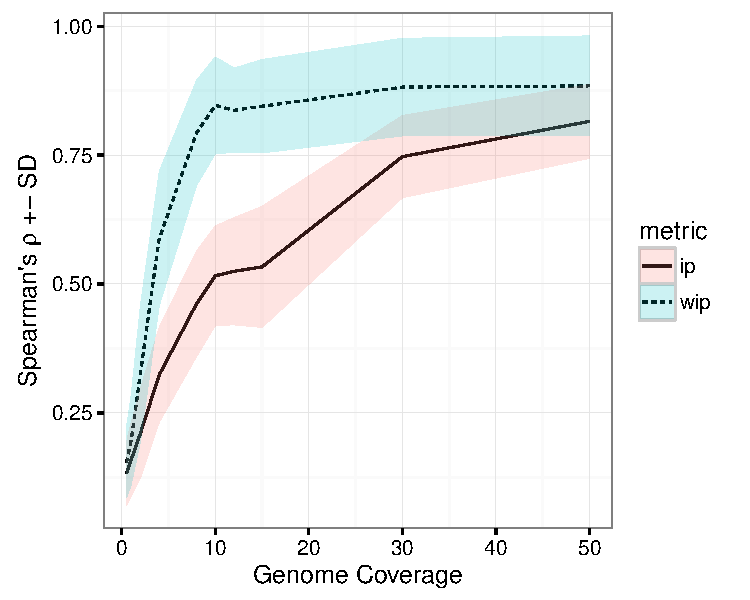
\includegraphics[width=0.4\linewidth]{coverage-vs-rho_50x.pdf}
  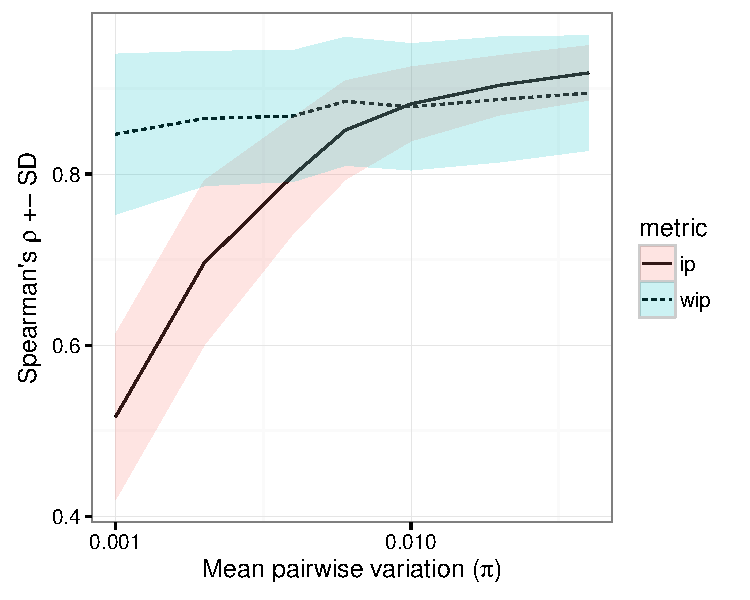
\includegraphics[width=0.4\linewidth]{pi-vs-performance.pdf}
\end{center}

\subsubsection*{Population structure detected}

Using a \textit{Chlamydomonas} population re-sequencing experiment
\autocite{flowers_whole-genome_2015}, we show \texttt{kWIP} can detect
population structure approximately as well as a state-of-the-art reference-based
variant calling pipeline.

\begin{center}
  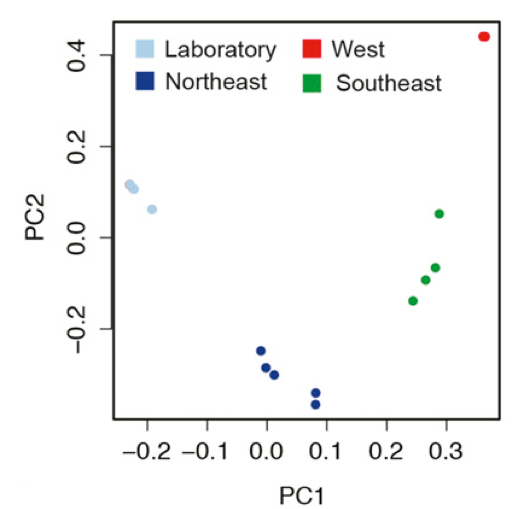
\includegraphics[width=0.34\linewidth]{flowers.png}
  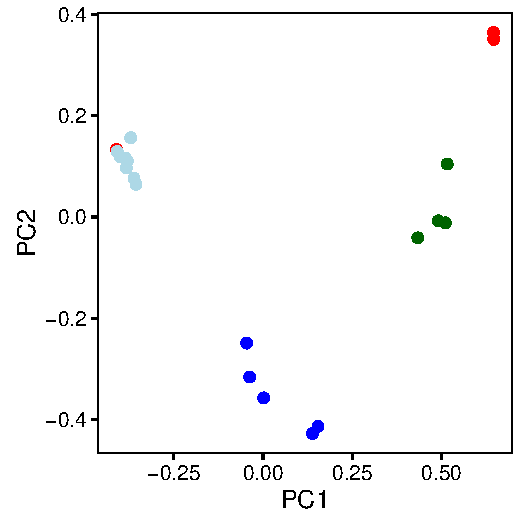
\includegraphics[width=0.32\linewidth]{chlamy.pdf}
\end{center}


\subsubsection*{Replicates are accurately clustered}

Using data from the 3000 Rice genomes sequencing project
\autocite{3k_rice_genomes_2014} we show weighting improves replicate clustering
accuracy. Representative example show below (erroneous clustering indicated by
red highlighting).

\begin{center}
  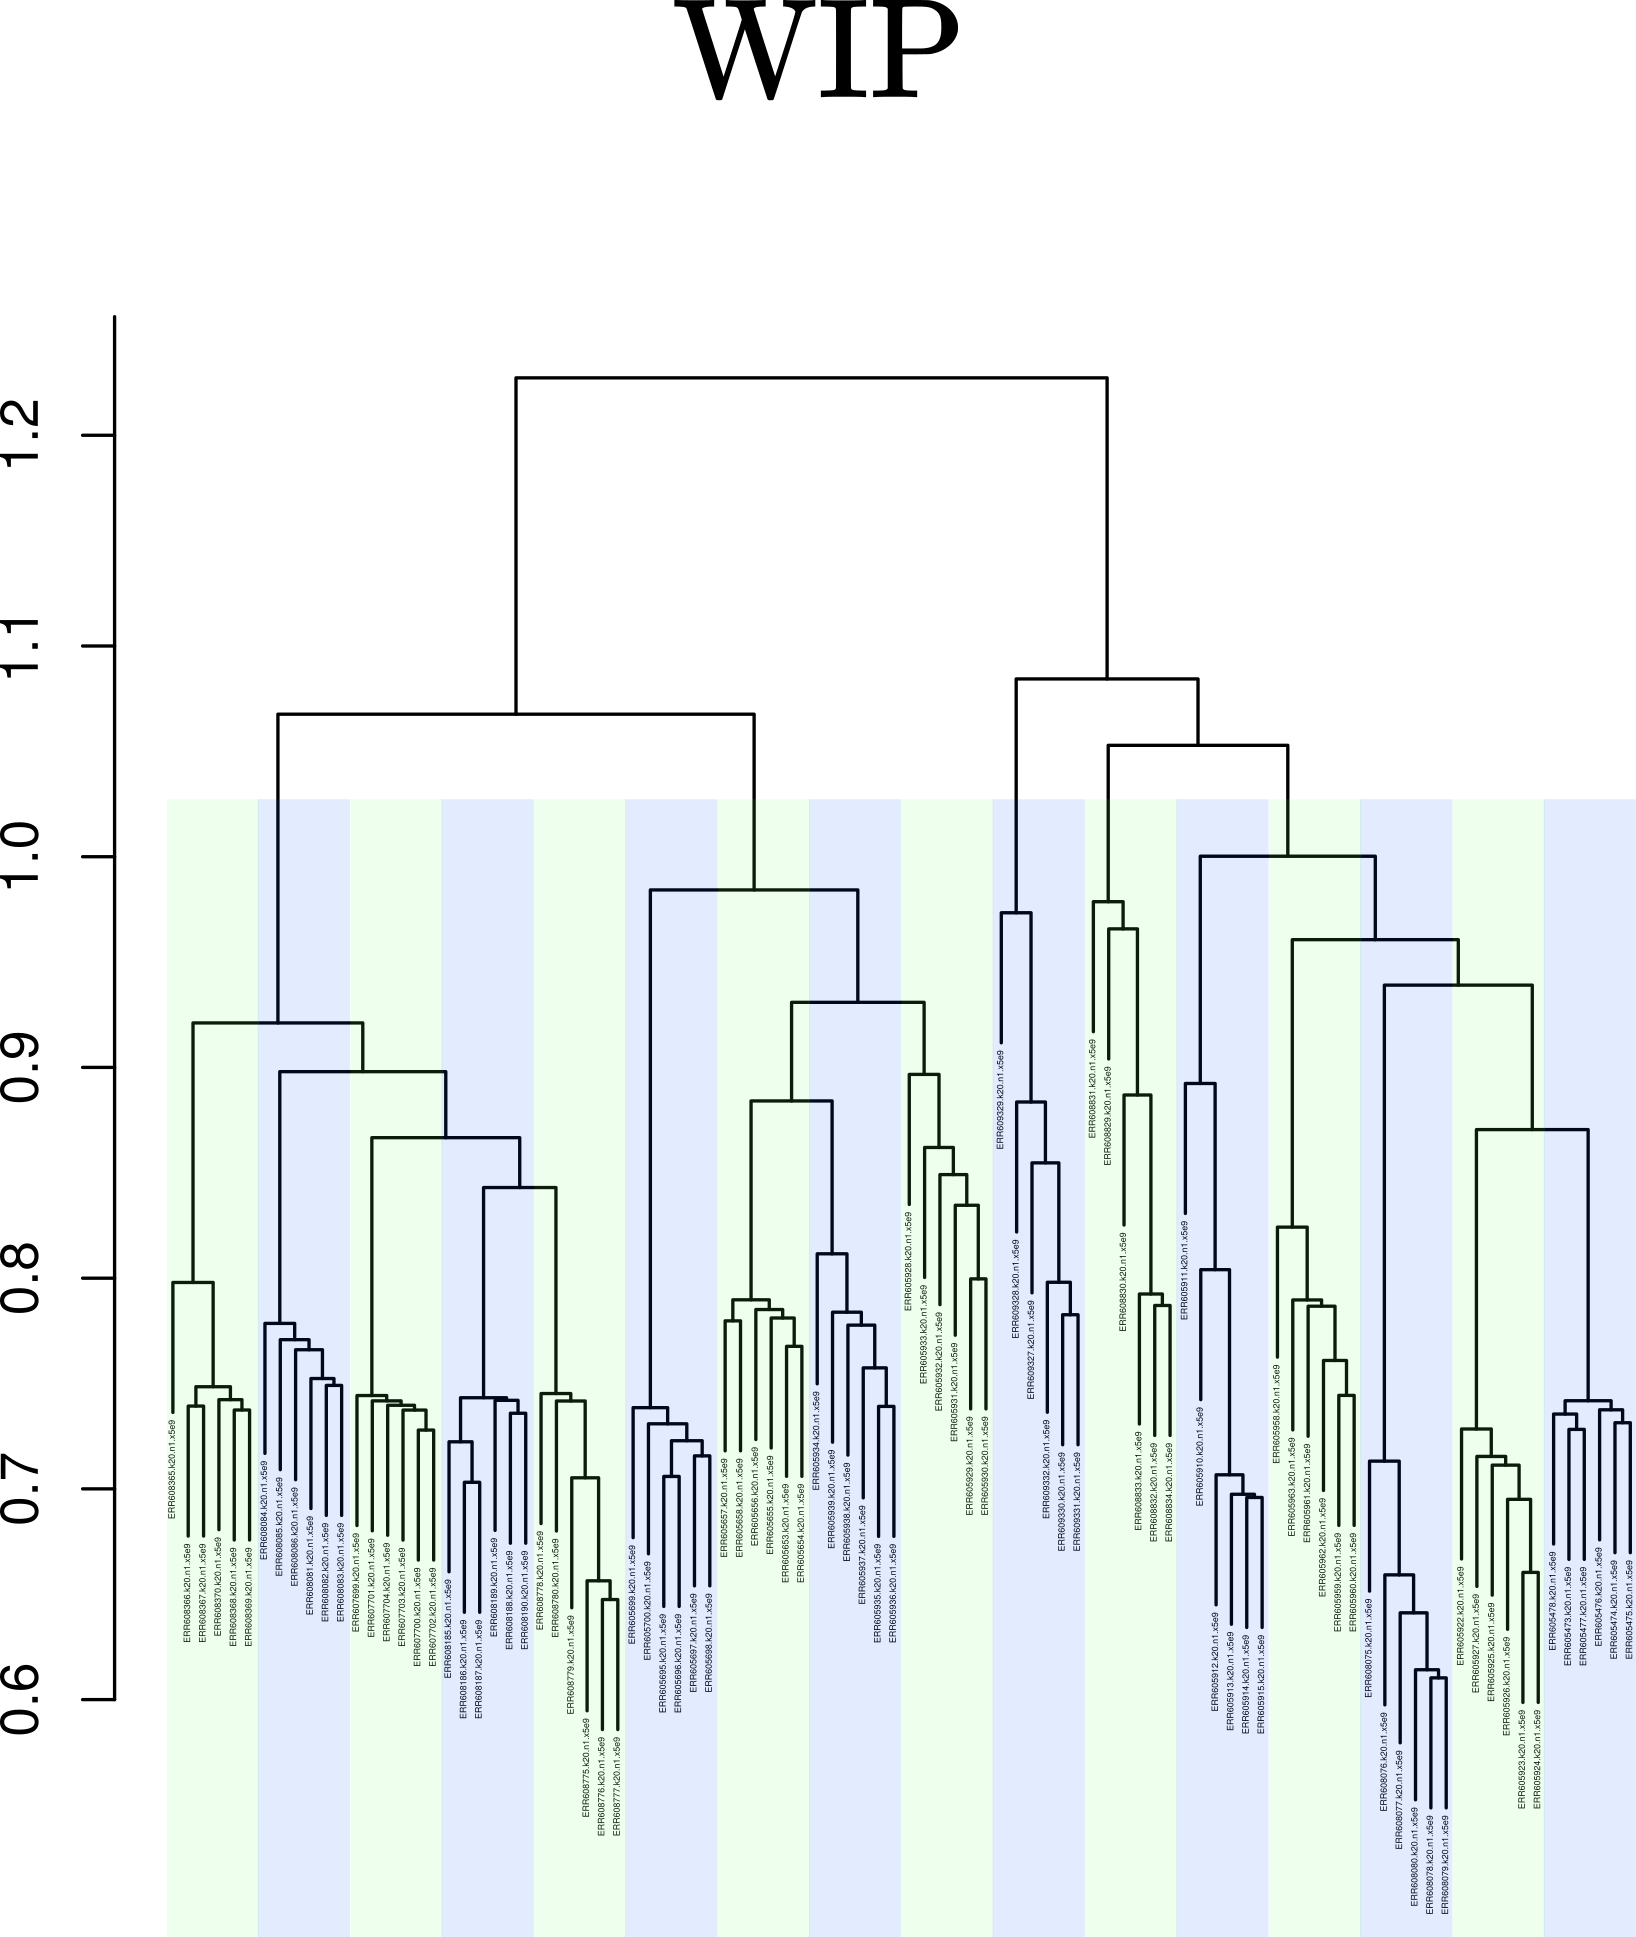
\includegraphics[width=0.3\linewidth]{rice-wip.png}
  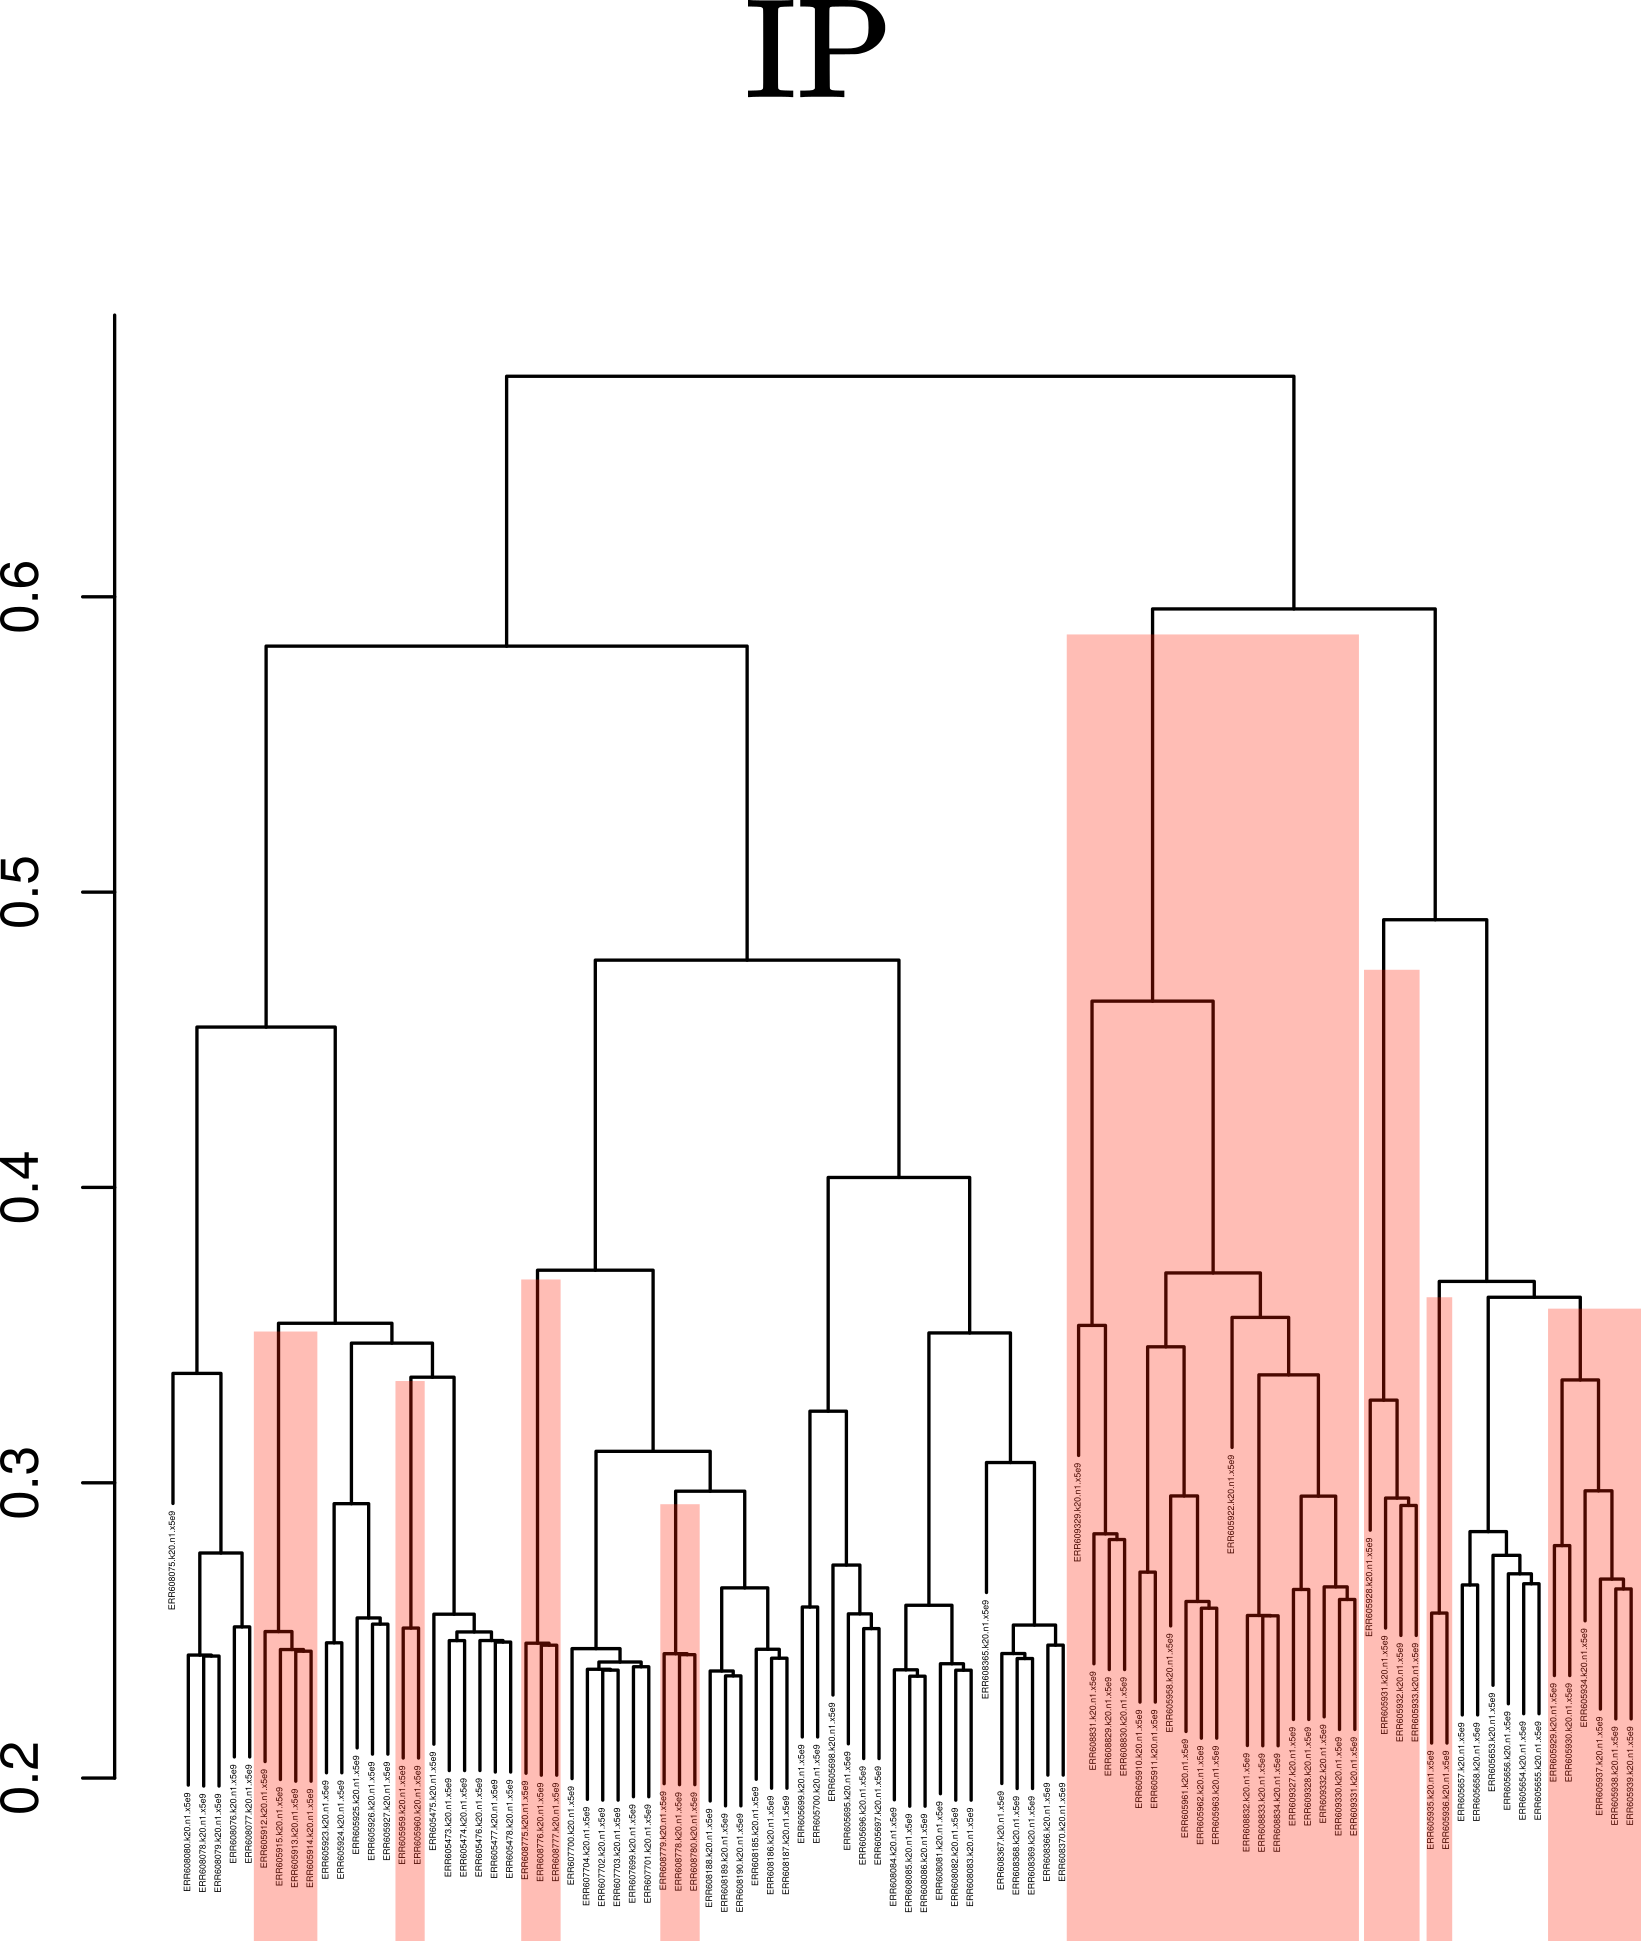
\includegraphics[width=0.3\linewidth]{rice-ip.png}
\end{center}


%------------------------------------------------------------------------------
%	CONCLUSIONS
%------------------------------------------------------------------------------

\color{ForestGreen}


\section*{Summary}
\Large
\texttt{kWIP}: a fast tool to determine approximate genetic relatedness
\begin{itemize}
  \item Entirely \textit{de novo} and alignment free
  \item Hashes $k$-mers into probabilistic data structures
  \item Calculates inner products between sample hashes
  \item Available from \url{https://github.com/kdmurray91/kwip} under the GNU GPL
\end{itemize}

\normalsize
\color{Black}

%------------------------------------------------------------------------------
%	FORTHCOMING RESEARCH
%------------------------------------------------------------------------------

\section*{Forthcoming Research}

A paper describing \texttt{kWIP} in more detail is in preparation. We plan to
deploy \texttt{kWIP} across several large-scale plant population genome
sequencing projects. An MPI-parallelised implementation is in preparation.

%------------------------------------------------------------------------------
%	ACKNOWLEDGEMENTS
%------------------------------------------------------------------------------

\section*{Acknowledgements}

We thank Sylvain For\^{e}t, Conrad Burden, Terry Neeman, Ben Kahler, Gavin
Huttley and Cameron Jack for comments or advice on algorithms and experiments
presented here.


%------------------------------------------------------------------------------
%	REFERENCES
%------------------------------------------------------------------------------
\tiny
\printbibliography
\normalsize

%------------------------------------------------------------------------------
\end{multicols}
\end{document}
